\chapter{Resum\'e en fran\c{c}ais}
\minitoc

\section{Introduction}
 Les \'etoiles naissent en groupe, lors de flamb\'ees de formation stellaire au sein de nuages mol\'eculaires. Les diff\'erentes \'etapes de cette formation stellaire sont pr\'esentes dans notre ciel: nuage mol\'eculaire froid, r\'egion d'\'emission HII peupl\'ee de coeur proto-stellaires, jeune amas enfoui (dans son gaz), jusqu'au stade \'evolu\'e d'un jeune amas d\'eposs\'ed\'e de son gaz primordial. Cette s\'equence \'evolutive de plusieurs millions d'ann\'ees se d\'eroule dans le ciel au fil des objets et r\'egions observ\'ees. 
 
La compr\'ehension de ce processus est cruciale pour appr\'ehender la formation stellaire en g\'en\'eral et m\^eme galactique. En effet, les amas globulaires sont consid\'er\'es comme des t\'emoins majeurs de la formation des galaxies. S\'epar\'es en populations bleues, \`a faible m\'etallicit\'e, et rouge \`a haute m\'etallicit\'e, les amas globulaires ont un lien complexe avec les fusions galactiques. Par exemple, des jeunes amas massifs, ou YMC (Young Massive Clusters), sont observ\'es dans des galaxies en train de fusionner, comme les Antennes. Ces objets sont consid\'er\'es comme de futurs amas globulaires.

Or notre compr\'ehension de ces amas reste incompl\`ete. Longtemps consid\'er\'es comme les syst\`emes homog\`enes par excellence, un seul \^age, une seule m\'etallicit\'e, plusieurs s\'equences stellaires ont r\'ecemment \'et\'e observ\'ees cohabitant au sein des m\^emes amas. Ces populations multiples pourraient s'expliquer par le processus de formation des amas. Le gaz mol\'eculaire dont les \'etoiles \'emergent et les r\'egions de formations stellaires sont profond\'ement sous-structur\'es, les filaments et grumeaux sont la normes. Seuls les amas plus \^ag\'es ont une structure lisse, concentr\'ee et sym\'etrique. Cela implique une \'evolution dynamique, plusieurs grumeaux doivent fusionner pour former ces amas. Si ces grumeaux ont des m\'etallicit\'es et/ou des \^ages diff\'erents, cela pourrait expliquer les populations multiples des amas globulaires.



\begin{figure}
\center
    \centering
    \begin{subfigure}[b]{0.48\textwidth}
    	\centering
        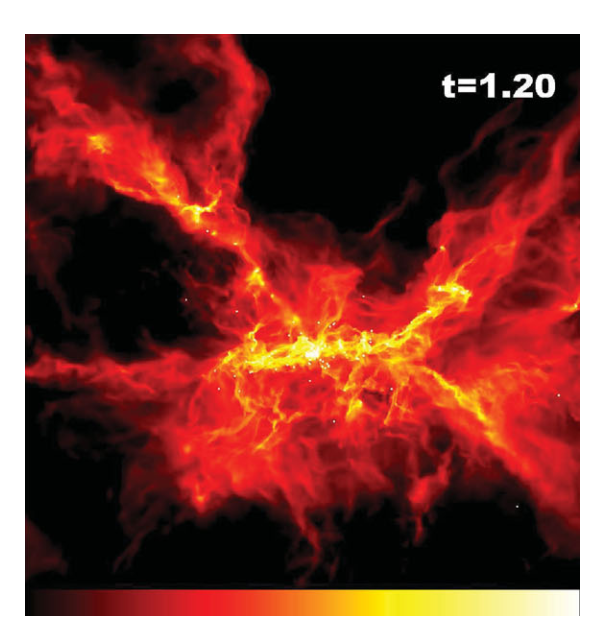
\includegraphics[width=0.9\textwidth]{Figures/0_bate2012.png}
        \caption{Simulation hydrodynamique}
        \label{Fig:resume_bate2012}
    \end{subfigure}
    \begin{subfigure}[b]{0.48\textwidth}
        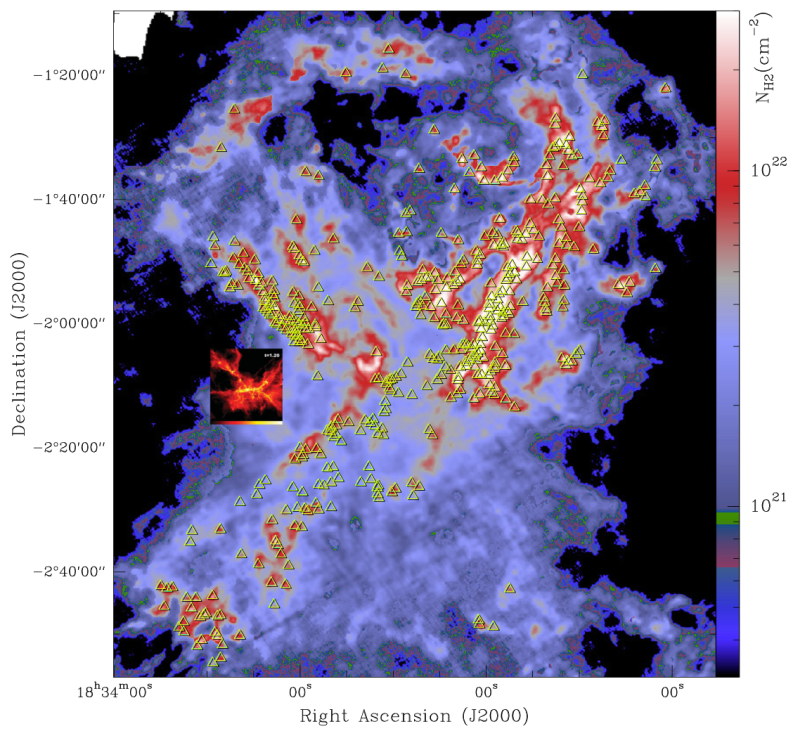
\includegraphics[width=\textwidth]{Figures/0_aquila_bate.png}
        \caption{Observation: gaz et proto-\'etoiles}
        \label{Fig:resume_aquila_bate2012}
    \end{subfigure}
\caption{(a): comparaison entre une simulation hydrodynamique de formation stellaire tir\'ee de \cite{Bate2012}; (b): observations Herschel infrarouge du complexe de formation stellaire Aquila, tir\'ee de \cite{Konyves2010}. La densit\'e de colonne correspond aux niveaux de rouge et jaune \`a gauche, et aux niveaux de bleu et rouge \`a droite. La simulation fait $\sim$ 0.6 parsecs de c\^ot\'e et les observations, en consid\'erant l'estimation de distance prise par les auteurs, s'\'etend sur 7 parsecs. La simulation a \'et\'e ins\'er\'ee \`a droite pour comparer les \'echelles.}
\label{Fig:resume_clumps}
\end{figure}

Les simulations hydrodynamiques permettent de reproduire la formation stellaire et d'observer l'\'evolution de ces sous-structures. H\'elas, elle sont souvent co\^uteuses en temps et en ressources de calcul, et sont limit\'ees \`a des petit syst\`emes (souvent un grumeau isol\'e), \'evoluant pour un temps assez court. Pour pouvoir aller plus loin et prendre en compte l’int\'eraction entre les grumeaux, il est possible de prendre le relai avec des simulations \`a N-corps, en consid\'erant le gaz comme \'evacu\'e par les \'etoiles. Les simulations \`a N-corps sont moins gourmandes en ressources et permettent de mod\'eliser de bien plus grand syst\`emes sur des \'echelles de temps plus importantes.

Pour pouvoir simuler l'\'evolution de ces syst\`emes de mani\`ere r\'ealiste avec des simulations N-corps, il est n\'ecessaire de g\'en\'erer des conditions initiales r\'ealistes: sous-structur\'ees, sous-virielles comme le montrent plusieurs observations de jeunes amas. Plusieurs m\'ethodes existent pour g\'en\'erer ce genre de syst\`eme: correlation au gaz dans une simulation hydrodynamique, grumeaux de Plummer ou croissance d'arbre fractale. Ces m\'ethodes se basent sur des simulations hydrodynamiques et restent co\^uteuse, ou produisent des syst\`emes avec une structure  artificielle dans l'espace des phases, ne prenant pas en compte l'\'etat dynamique du syst\`eme.

\paragraph*{}
Mon travail de th\`ese s'est concentr\'e sur la cr\'eation et l'exploration d'une nouvelle m\'ethode de g\'en\'eration de conditions initiales pour simuler de jeunes amas sous-structur\'es \`a travers des simulations N-corps. Cette m\'ethode est l'expansion de \HubLem, elle se base sur l'expansion radiale d'un syst\`eme uniform pour laisser des surdensit\'es naturelles se developper et construire des grumeaux auto-coh\'erents dans l'espace des phases.

Dans ce travail, j'approche d'abord la m\'ethode de mani\`ere analytique, d\'egageant les \'equations qui gouvernent l'expansion du syst\`eme. J'analyse ensuite des r\'ealisations num\'eriques du mod\`ele, en comparant les grumeaux aux observations et simulations hydrodynamiques. Je prend ensutie ce mod\`ele comme conditions initiales pour \'etudier la relaxation violente d'un amas jeune, sous-viriel et sous-structur\'e.

Dans un deuxi\`eme temps, je change d'\'echelle dynamique et m'int\'eresse aux \'etoiles binaires et \`a l'\'evolution de leur population dans ce genre de syst\`eme sous-structur\'es. J'analyse la population spontan\'ee apparaissant dans les mod\`eles de \HubLem, puis j'injecte des binaires suppl\'ementaires pour me rapprocher des tendances des populations de binaires observ\'ees dans le champs galactique. Enfin, je laisse les mod\`eles \'evoluer comme pr\'ec\'edemment pour explorer l'influence des sous-structures et de l'effondrement sur la population de binaires.


\section{Partie I: Le mod\`ele fragment\'e et son \'evolution}


Pour g\'en\'erer un mod\`ele fragment\'e de \HubLem, on g\'en\`ere tout d'abord une sph\`ere uniforme en tirant des \'etoiles d'une fonction de masse stellaire, Salpeter ou $L_3$. On attribue ensuite des vitesses radiales selon
\begin{equation}
\bold{v} = \Hub_0 \bold{r},
\end{equation}
analogue au champs de vitesse observ\'e pour les galaxies dans l'univers, $\Hub_0$ \'etant l'\'equivalent de la constante de Hubble mais dont la valeur est ici libre. On laisse ensuite ce syst\`eme \'evoluer \`a travers un int\'egrateur N-corps.

Pour mon travail, j'ai utilis\'e NBODY6, cr\'e\'e par Sverre Aarseth. Ce choix a \'et\'e motiv\'e par les nombreux avantages du code: c'est un int\'egrateur collisionel, capable de traiter des interaction proches et des \'etoiles binaires sans adoucir le potentiel, il poss\`ede de nombreuses optimisations algorithmiques qui font de lui un des int\'egrateurs N-corps les plus rapides, et enfin il poss\`ede une version GPU, permettant d'acc\'el\'erer encore plus les simulations pour des nombres de particule suffisammen \'elev\'es.

J'ai \'egalement developp\'e un environnement python, \textit{StarFiddle}. Il s'agit d'une interface python pour NBODY6 coupl\'e \`a un environnement d'analyse pour les r\'esultats de simulation N-corps. StarFiddle poss\`ede de nombreux modules: graphes 3d interactifs, calcul des \'energies \`a travers une librairie Cuda, d\'etection des \'etoiles binaires ou des grumeaux dans une simulation, etc. Il est disponible sur \href{https://github.com/dorvaljulien/StarFiddle}{GitHub}.

Pendant l'expansion, les \'etoiles massives tendent \`a attirer des \'etoiles plus l\'eg\`ere, faisant croitre les sur-densit\'es initiales dans le mod\`ele. On peut montrer par le calcul que la constante $\Hub_0$ doit \^etre inf\'erieure \`a $\sqrt{2}$ pour avoir un syst\`eme li\'e et que l'expansion stoppe \`a un temps donn\'e. Ce temps augmente rapidement lorsque qu'on se rapproche de cette valeur limite.

Il est possible de faire une analyse en perturbation du syst\`eme en expansion en consid\'erant des surdensit\'es en coquille spheriques. Cela nous apprend que les surdensit\'es devraient d'abord converger en r\'egime lin\'eaire, puis rentrer dans une phase d'\'evolution collisionelle, d'o\`u peut \'emerger une s\'egr\'egation de masse.


\begin{figure}
\begin{center}
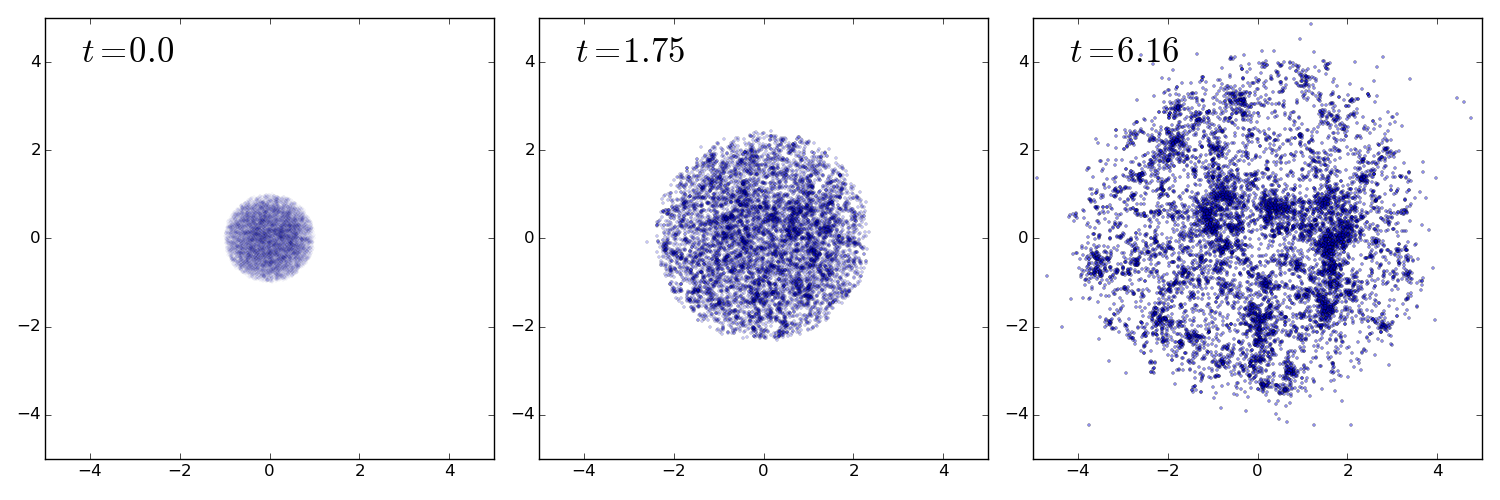
\includegraphics[width=\textwidth]{Figures/2_fragmentation}
\caption[Fragmentation of a \HubLem model]{Progressive fragmentation through the Hubble expansion. The left panel shows the initial uniform sphere; the middle panel, an intermediate step, slightly fragmented with a slowed down expansion; the right panel is the final stage, when the expansion has stopped and the fragmentation is fully developed. N=10000 particles were used in this N-body model, with $\Hub_0 = 1.0$. Time and coordinates are in H\'enon units.}
\label{Fig:resume_fragmentation}
\end{center}
\end{figure}


\paragraph*{}
L'analyse des mod\`eles fragment\'es obtenus num\'eriquement \`a travers NBODY6 n\'ecessite de pouvoir isoler les grumeaux et les analyser. Pour cela, j'ai adapt\'e la m\'ethode utilis\'ee par \cite{Maschberger2010} pour isoler les surdensit\'es dans leur simulation hydrodynamique. on construit d'abord l'arbre couvrant de poid minimal, où MST (Minimum Spanning Tree) du syst\`eme, puis en coupant toutes les branches plus longues qu'une certaine longueur, on consid\`ere tous les syst\`emes li\'es et isol\'es comme des grumeaux. J'ai fix\'e le seul param\`etre libre, la longueur de coupure, en maximisant le nombre de grumeaux d\'etect\'es. Ce choix donne des grumeaux coh\'erents, et un test sur des modèles artificiellement sous-structurés a confirm\'e que l'algorithme permettait de retrouver une distribution th\'eorique de grumeaux inject\'ee dans un syst\`eme.

L'exploration des diff\'erents param\`etres et la r\'ealisation d'une multitude de mod\`ele de \HubLem a permis de d\'egager les caract\'eristiques suivantes: la fonction de masse des grumeaux est peu sensible au nombre total d'\'etoiles N ou \`a $\Hub_0$, mais elle est en revanche d\'ependante aux bornes de la fonction de masse stellaire. Une masse stellaire maximum \`a 100 $\Mo$ donne une queue de fonction de masse de grumeau en loi de puissance avec un index proche de -1, lorsque cette masse maximum descend \`a 20$\Mo$, la queue de la distribution accentue sa pente, l'index descend \`a -1.7. Le pic de la distribution se maintient \`a $\sim$ 20 $\Mo$. Des simulations avec masse stellaire unique ont about \`a une fonction de masse en loi de puissance à -4.

Cela souligne l'importance majeure des \'etoiles massives dans la fragmentation. Cette importance est confirm\'ee par les r\'esultats suivants. Les grumeaux ont comparativement plus d'\'etoiles massives que les \'etoiles dites "du champs", celles n'\'etant pas d\'etect\'ees comme faisant partie d'un grumeau. la diff\'erence entre les distributions stellaires rappelle celle observ\'ees entre le champs galactique et les amas stellaires, voir Fig.~\ref{Fig:resume_ClumpMembers}. De plus, la relation  $m_{max} - M_{grumeau}$ dans nos syst\`eme montre que $m_{max}$ est généralement supérieur à ce que l'on pourrait attendre d'un tirage direct de la fonction de mass initiale. Cela recouvre la tendance observ\'ee dans des amas jeunes enfouis. Enfin, en utilisant la m\'ethode de rang radial pour mesurer la s\'egr\'egation de masse, en accord avec \cite{Maschberger2010}, nous trouvons une tendance g\'en\'erale \`a la s\'egr\'egation dans nos grumeaux, similaire \`a ce qui est mesur\'e dans les sur-densit\'es des simulations hydrodynamiques. Cette ségrégation semble concentrée, statistiquement, sur les trois étoiles les plus massives de chaque grumeaux.


\begin{figure}
\begin{center}
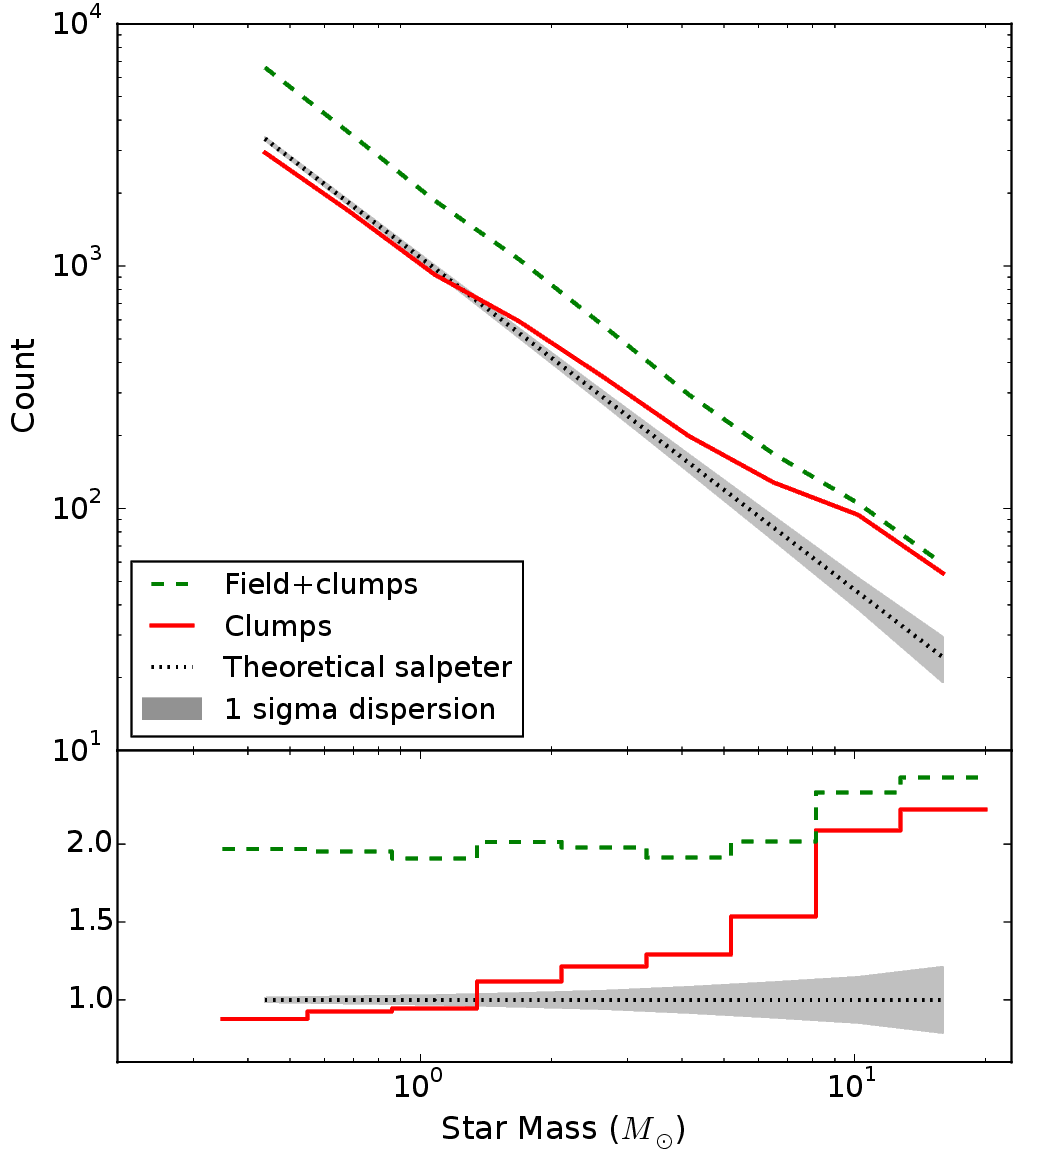
\includegraphics[width=0.75\textwidth]{Figures/2_ClumpMembers}
\caption{ En haut: fonction de masse des étoiles appartenant à un grumeau (ligne continue rouge), et celle des étoiles hors des grumeaux (line continue bleue). L'attente statistique d'après une fonction de masse de Salpeter est montrée en pointillés noirs, et la dispersion de ce tirage en zone grisée. Les pointillés verts correspondent à la distribution de tout l'amas. En bas: même données normalisés à l'attente de Salpeter.}
\label{Fig:resume_ClumpMembers}
\end{center}
\end{figure}


\paragraph*{}
Ces r\'esultats valident les mod\`eles de \HubLem comme \'etant des conditions initiales adapt\'ees pour simuler l'\'evolution dynamique de jeunes amas stellaires. Nous laissons ces mod\`eles \'evoluer et subir une relaxation violente avant d'atteindre un \'etat virialis\'e de quasi-\'equilibre. Pour pouvoir d\'egager l'influence des sous-structures sur cette \'evolution, nous avons \'egalement simul\'e la relaxation de mod\`eles uniformes froids. Les étapes des effondrements de ces modèles sont montrées dans la Fig.~\ref{Fig:resume_collapse}. Tous les mod\`eles ont \'et\'e simul\'es jusqu'\`a 40 unit\'es de temps H\'enon, ce qui correspond ici \`a $\sim$ 16 temps de travers\'ee du syst\`eme, mais bien moins qu'un temps de relaxation.


\begin{figure}
\begin{center}
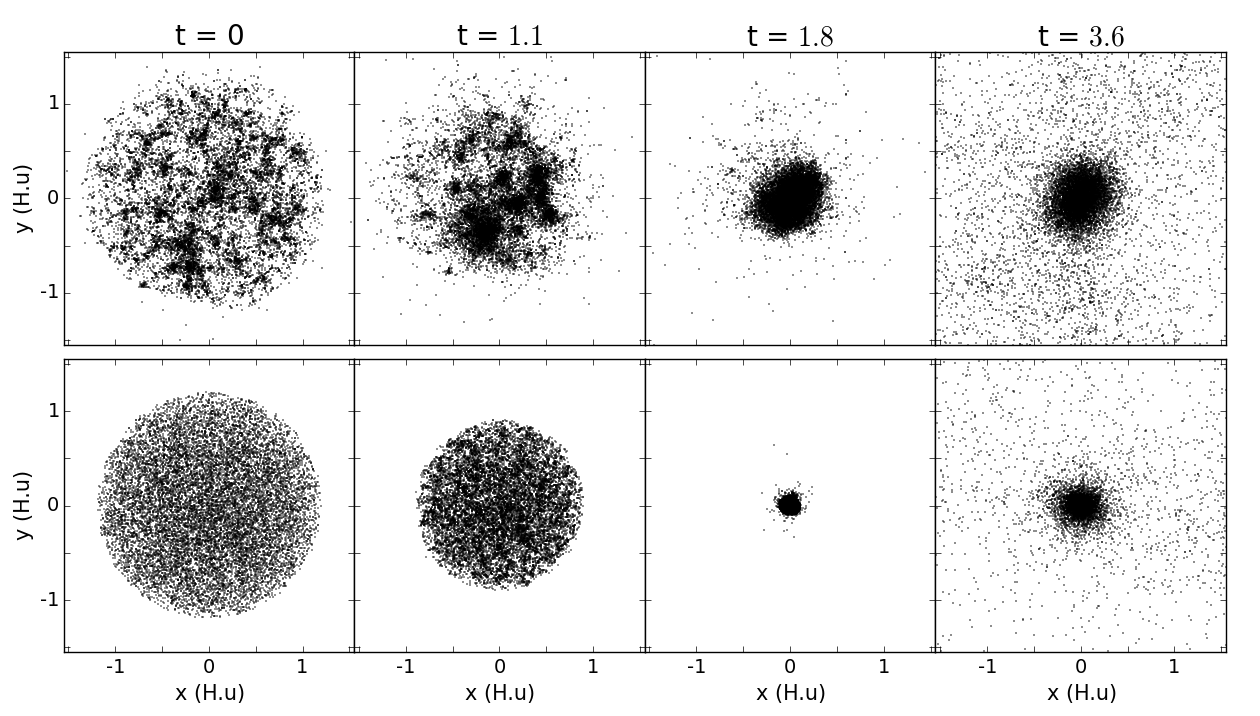
\includegraphics[width=\textwidth]{Figures/3_collapse}
\caption{Systèmes fragmentés de \HubLem (en haut) et uniformes (en bas) à plusieurs étapes de l'effondrement. Les étapes sont, de gauche à droite: conditions initiales; pendant l'effondrement; rebond; juste après l'effondrement. Le temps est donné en unités H\'enon.}
\label{Fig:resume_collapse}
\end{center}
\end{figure}




\begin{figure}
\begin{center}
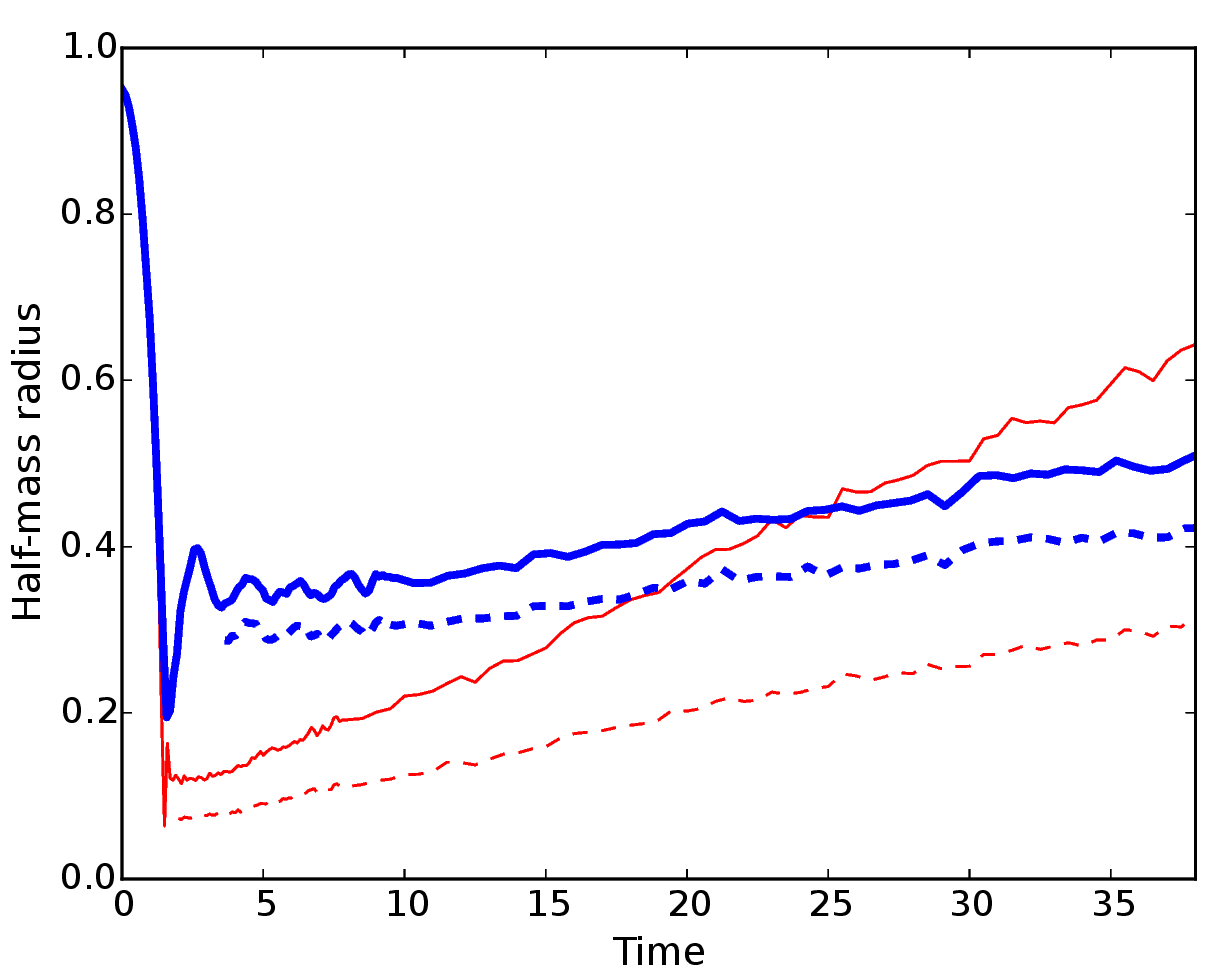
\includegraphics[width=0.7\textwidth]{Figures/3_Rhm_global}
\caption{Rayon de mi-masse en fonction du temps pour deux systèmes subissant un effondrement froid: un modèle uniforme (ligne rouge continue) et un modèle fragmenté de \HubLem (ligne bleue continue). Les rayons de mi-masse et le temps sont en unité H\'enon, avec $1 t_{Henon} =  0.13 \Myr$. Les lignes en pointillés correspondent au systèmes auxquels ont été soustraits les étoiles éjectés par le rebond.}
\label{Fig:resume_Rhm_global}
\end{center}
\end{figure}



L'effondrement des mod\`eles de \HubLem est plus doux que celui des syst\`emes uniformes en raison des grumeaux. En cons\'equence, le syst\`eme central est moins dens\'e. Les syst\`emes uniformes \'ejectent deux fois plus d'\'etoiles au rebond que les mod\`eles fragment\'es. Nous avons developp\'e une m\'ethode d'extraction des \'etoiles \'eject\'ees permettant le retrait d'\'etoiles marginalement li\'ees au syst\`eme. En se concentrant sur les syst\`emes li\'ees, le coeur plus concentr\'e des syst\`emes uniformes acc\`el\`ere leur \'evolution \`a deux-corps, ils s'\'etendent pour au final avoir une structure spatiale comparable aux syst\`emes fragment\'es \`a t = 40 H.u. Les rayons de mi-masse des modèles sont tracés en fonction du temps sur la Fig.~\ref{Fig:resume_Rhm_global}.

En s\'eparant les \'etoiles des syst\`emes par masse et en repr\'esentant l'\'evolution de leur r\'epartion dans le syst\`eme, on remarque que les syst\`emes uniformes tendant \`a developper une s\'egr\'egation de masse plus important que les syst\`emes fragment\'es en fin de simulation. Pourtant, juste apr\`es l'effondrement, les mod\`ele de \HubLem sont plus s\'egr\'eg\'es, et cette s\'egr\'egation est concentr\'ee sur les \'etoiles les plus massives. Cette s\'egr\'egation sp\'ecifique est h\'erit\'ee des grumeaux, dans lesquel le faible nombre d'\'etoiles pouvaient difficilement d\'evelopper une s\'egr\'egation r\'eguli\`ere, et se maintient dans l'\'evolution du syst\`eme virialis\'e, en contraste avec la s\'egr\'egation des syst\`emes uniformes, plus \'etal\'ee sur le spectre de masse stellaire. Dans un v\'eritable amas stellaire, cela augmenterait les gradients de couleurs dans le coeur, en comparaison d'un syst\`eme provenant d'un effondrement plus uniforme.



\section{Partie II: Les \'etoiles binaires dans les amas sous-structur\'es}

Dans la deuxi\`eme partie de cette th\`ese, je me suis concentr\'e sur les \'etoiles binaires et le sort des populations de binaires dans les amas jeunes, sous-structur\'es et sous-viriels. Certains auteurs s'\'etaient d\'ej\`a sp\'ecifiquement pench\'es sur ce probl\`eme \citep{Parker2011}, mais \`a travers des mod\`eles fractaux, qui manquent la coh\'erence dynamique des syst\`emes de \HubLem, et pour des nombres d'\'etoiles limit\'es \`a 1 ou 2 milliers. Le but de cette deuxi\`eme partie \'etait d'explorer l'influence de la dynamique collisionelle \`a l’int\'erieur des grumeaux sur les syst\`emes binaires, ainsi que celle de l'effondrement et de son champs de mar\'ee li\'e au nombre total d'\'etoile.

J'ai d\'evelopp\'e un algorithme de d\'etection d'\'etoile binaire dans les simulation \`a N-corps reposant sur une structure de donn\'ee appel\'ee arbre KD. La recherche de paire d'\'etoile li\'ee est la premi\`ere phase de l'algorithme, et cette recherche s'effectue, pour chaque \'etoile, parmi les voisins directs. L'arbre KD permet, une fois qu'il a \'et\'e construit, d'effectuer des recherches de voisins $\log(N)/N$ plus rapidement qu'en force brute. Une fois que deux \'etoiles sont d\'etect\'ees comme li\'ees, elles doivent d\'efinir une densit\'e plus importante que celle cr\'e\'e par les voisins directs. Si c'est le cas, elles sont confirm\'ees comme binaires. Cet algorithme a \'et\'e test\'e et son param\`etre libre valid\'e en ins\'erant une population de binaire connue dans un amas de King et en \'evaluant la solidit\'e des syst\`emes retourn\'es par l'algorithme.



\begin{figure}
\center
    \centering
    \begin{subfigure}[b]{0.48\textwidth}
    	\centering
        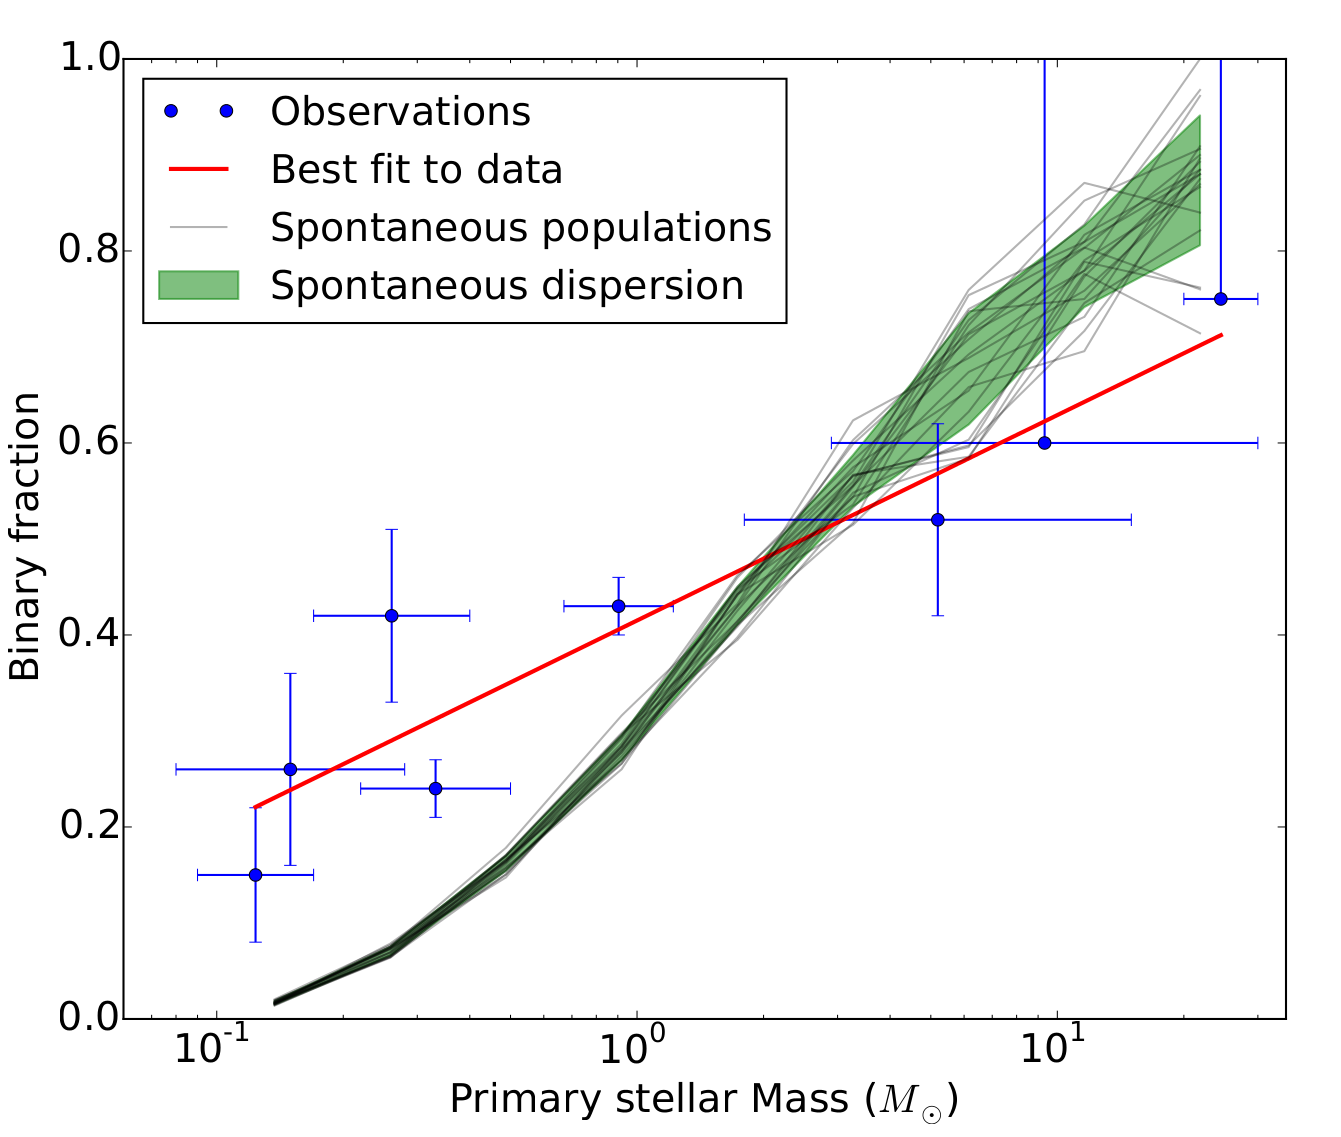
\includegraphics[width=\textwidth]{Figures/5_spontaneous_primarymass}
        \caption{Population spontan\'ee}
        \label{Fig:resume_spont}
    \end{subfigure}
    \begin{subfigure}[b]{0.48\textwidth}
        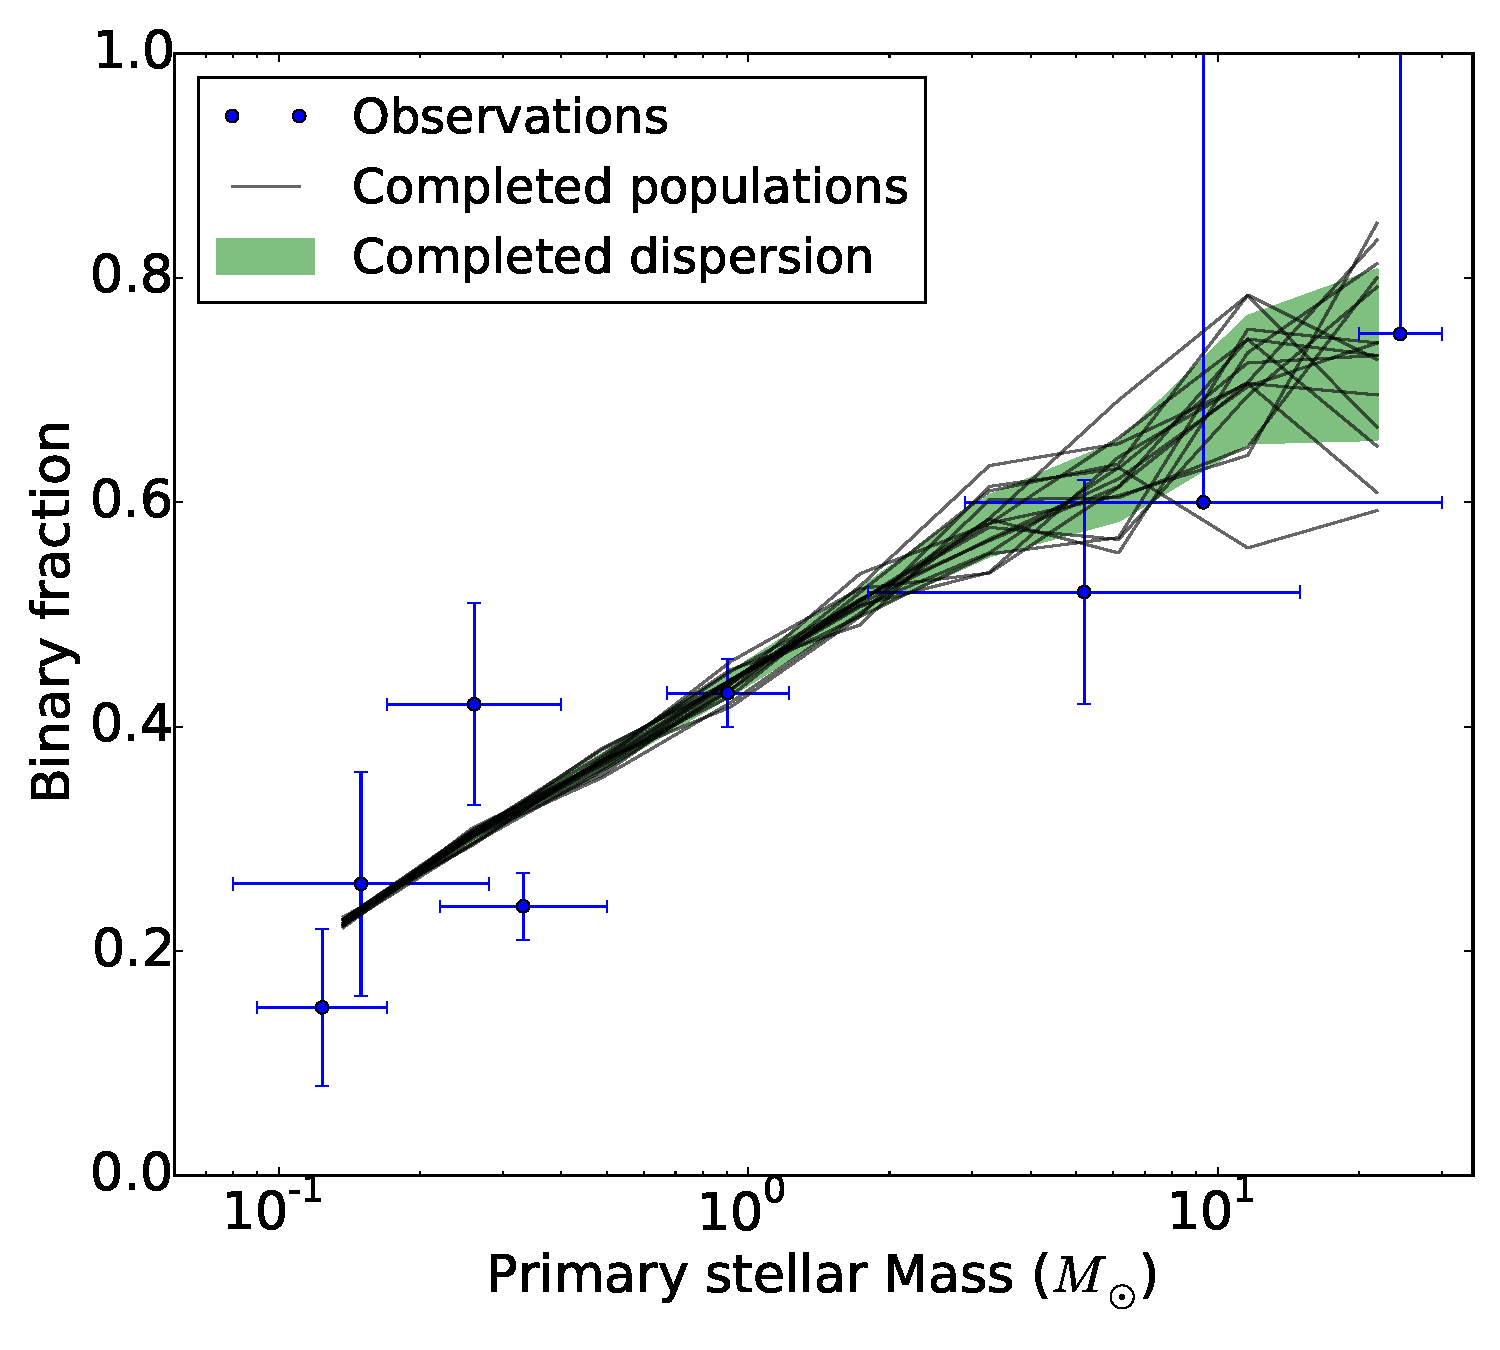
\includegraphics[width=\textwidth]{Figures/5_completed_primarymass}
        \caption{Population compl\'et\'ee}
        \label{Fig:resume_comp}
    \end{subfigure}
\caption{ Fraction de binaire en fonction de la masse primaire. Les r\'esultats sont moyenn\'es sur 20 mod\`eles diff\'erents, les zones color\'ees montrent la dispersion \`a 1 $\sigma$. Des binaires \`a faible masse primaire ont \'et\'e inject\'ee pour se rapprocher des observations dans la figure de droite.}
\label{Fig:resume_binpop}
\end{figure}


L'application de l'algorithme aux syst\`emes fragment\'es par la m\'ethode de \HubLem a r\'ev\'el\'e l'existence d'une population de binaire spontan\'ees, form\'ees pendant l'expansion initiale, pendant laquelle les \'etoiles proches \'etaient fortement corr\'el\'ees dans l'espace des phases. Cette population spontan\'ee poss\`ede une fraction de binaire croissante avec la masse de la primaire. Cette tendance est similaire \`a la distribution observ\'ee dans le champs galactique, mais la population spontan\'ee manque de syst\`emes avec des primaires de faible masse et des semi-axe majeur inf\'erieurs \`a $\sim$ 1000 AU, qui sont pourtant majoritaires dans les populations observ\'ees. J'ai d\'evelopp\'e une m\'ethode de compl\'etion de la population. La nature particuli\`ere des mod\`eles de \HubLem interdisait toute injection directe dans un syst\`eme existant. Les binaires doivent \^etre inject\'ees dans la sph\`ere uniforme initiale, en tant qu'objet unique portant la masse des deux composantes. Une fois l'expansion effectu\'ee et le syst\`eme fragment\'e, les binaires peuvent \^etre s\'epar\'ees et attribu\'ee des positions et vitesses internes coh\'erents avec leur caract\'eristiques. La population inject\'ee doit \^etre tir\'ee d'une distribution obtenue \`a travers un syst\`eme d'\'equations non linaires qui mod\'elisent la formation et la destruction de binaires au cours de l'expansion.

\paragraph*{}
Une fois ces mod\`eles compl\'et\'es, ils sont utilis\'es comme conditions initiales de la m\^eme mani\`ere que pr\'ec\'edemment: effondrement, relaxation violente et virialisation, puis \'evolution dynamique plus r\'eguli\`ere. Afin de d\'egager l'influence du nombre total d'\'etoiles, les mod\`eles sont construit avec N=1.5k, 5k, 20k et 80k \'etoiles. Pour explorer l'influence de la densit\'e , tous les mod\`eles ont \'et\'e construits avec deux densit\'es stellaires diff\'erentes: 6 \'etoiles/$\pc^3$ et 400 \'etoiles/$\pc^3$. Ces valeurs sont tir\'es des observations de \cite{King2012a} et sont repr\'esentatives des extr\^emes observ\'es dans les r\'egions de formation stellaires.

\begin{figure}
\begin{center}
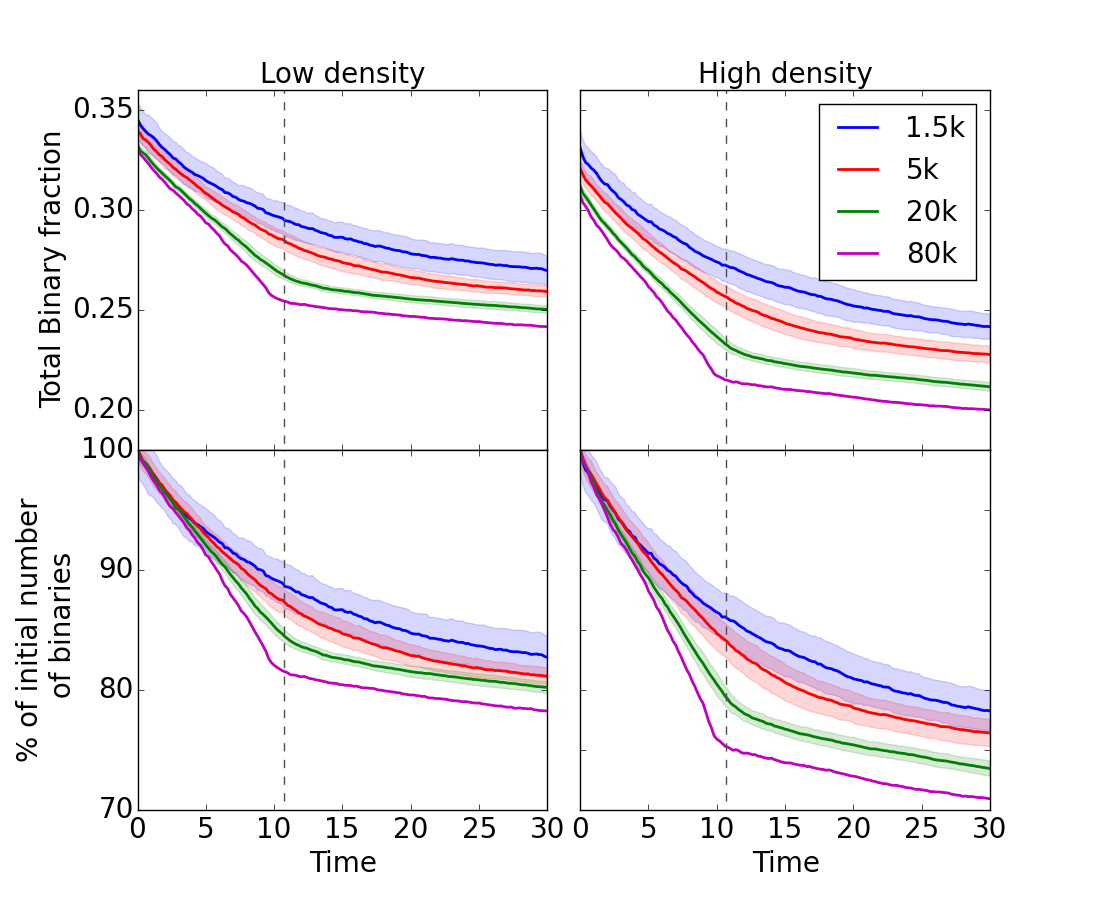
\includegraphics[width=0.8\textwidth]{Figures/6_TotBinFrac_vs_time_dispersion}
\caption{\'Evolution de la fraction de binaire totale (haut) et du nombre total de binaires en pourcentage de la population initiale (bas). La ligne verticale en pointill\'es indique le point d'effondrement le plus profond. Les donn\'ees sont moyenn\'ees sur tous les exemplaires de chaque mod\`ele, et les zones color\'ees montrent la dispersion \`a 1 $\sigma$.}
\label{Fig:resume_TotBinFrac}
\end{center}
\end{figure}

En mesurant la fraction total de binaires au cours du temps, on voit que les grumeaux d\'etruisent 10 fois plus de binaires par unit\'e de temps que le syst\`eme viriali\'e post-effondrement. Ces deux r\'egimes sont d'autant plus clairs que le nombre total d'\'etoiles est \'elev\'e. Gr\^ace aux puits de potential plus profond atteint par les amas avec 80k \'etoiles, ces derniers d\'etruisent deux fois plus de binaires que ceux avec 1.5k \'etoiles. La plupart des binaires avec des semi-axes majeurs sup\'erieur \`a 1000 AU sont d\'etruites, alors que celles plus courtes que $\sim$ 100 AU sont assez peu affect\'ees. Une faible tendance est observ\'ee, les amas avec plus d'\'etoiles atteignent et d\'etruisent des binaires l\'eg\`erement plus s\'err\'ees, mais cette tendance est plus faible que ce qu'un raisonnement analytique pourrait pr\'edire. Cette diff\'erence est probablement due aux sous-structures qui perturbent l'effondrement. Les binaires avec des primaires peu massives sont pr\'ef\'erentiellement d\'etruites dans les grumeaux, pendant l'effondrement. Dans le m\^eme temps, les primaires massives survivent mieux, voir voient leur population augmenter dans les mod\`eles avec peu d'\'etoiles et un faible champs de mar\'ee. En revanche, une fois l'effondrement pass\'e et le syst\`eme virialis\'e, toutes les binaires sont affect\'ees de la m\^eme mani\`ere par l'\'erosion de leur population.

\paragraph*{}
L'inspection d\'etaill\'ee des populations finales r\'ev\`ele l'existence des binaires "extremes": plus larges ou plus serr\'ees que ce qui a \'et\'e inject\'e dans le syst\`eme. Les binaires tr\`es larges ont des semi-axes majeurs sup\'erieurs \`a $10^4$ AU et se forment dans le halo d'\'etoiles \'eject\'ees lors du rebond. En effet, c'est un milieu \`a faible densit\'e et aux vitesses corr\'el\'ees, semblable \`a l'expansion initiale qui a vu naître les binaires spontan\'ees.

\begin{figure}
\begin{center}
    \begin{subfigure}[b]{0.9\textwidth}
    	\centering
    	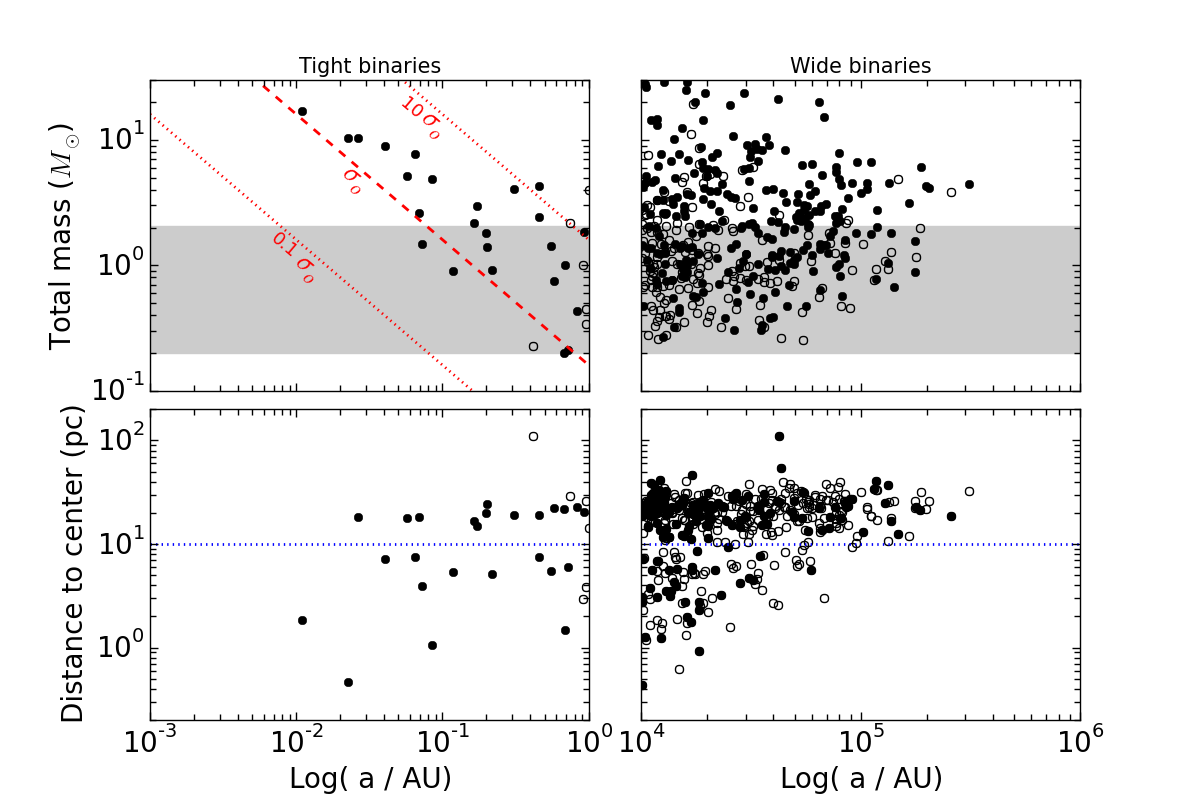
\includegraphics[width=0.85\textwidth]{Figures/6_extreme_binaries_LD}
        \caption{Mod\`eles \`a faible densit\'e}
        \label{Fig:6_extreme_LD}
    \end{subfigure}
    \begin{subfigure}[b]{0.9\textwidth}
    	\centering
    	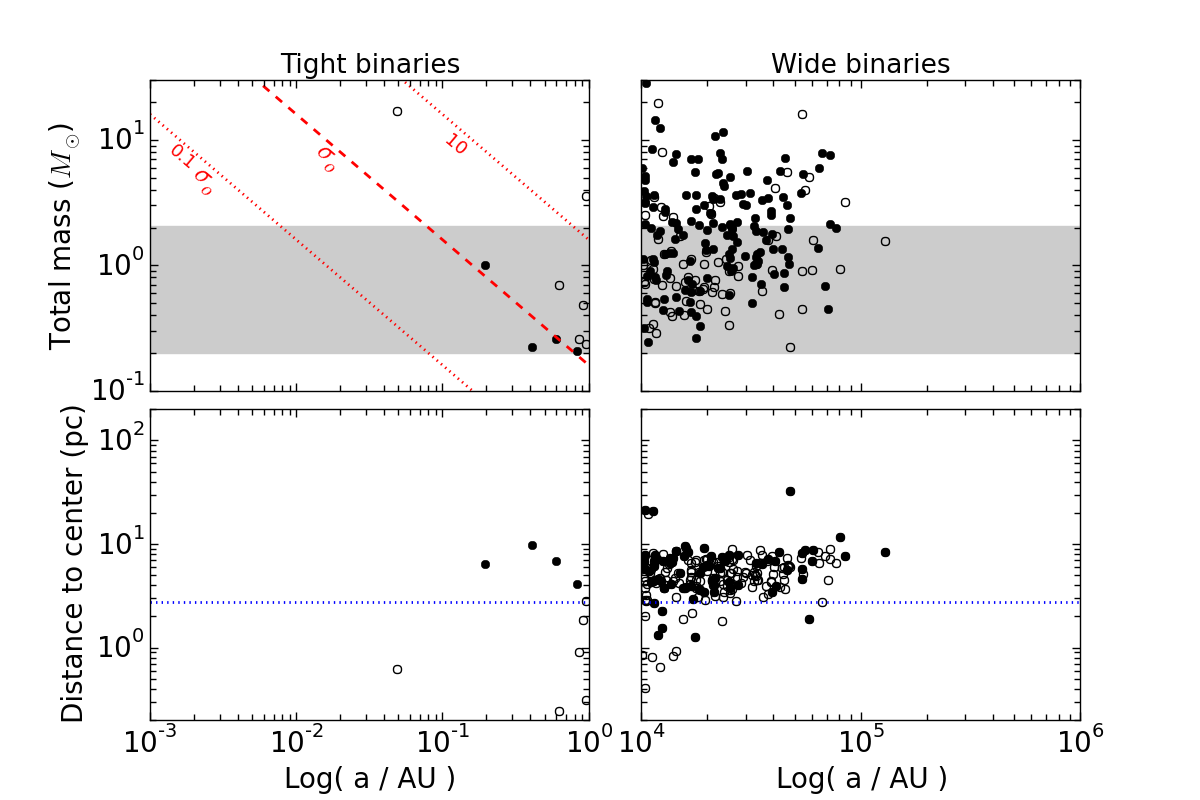
\includegraphics[width=0.85\textwidth]{Figures/6_extreme_binaries_HD}
        \caption{Mod\`eles \`a haute densit\'e}
		\label{Fig:6_extreme_HD}	        
    \end{subfigure}
\caption[Extreme tight and wide binaries]
{ \`A gauche: masse totale des binaires (en haut) et distance au centre de l'amas (en bas) pour les binaires plus serr\'ees que 1~AU \`a la fin de la simulation. \`A droite: m\^eme structure, pour les binaires plus large que $10^4$ AU. (a) repr\'esente les donn\'ees tir\'ees des simulations \`a faible densit\'e stellaire, et (b) celles tir\'ees des simulations \`a haute densit\'e. La zone gris\'ee sur les figures repr\'esentent la zone où 90\% des binaires devraient se trouver si les composantes \'etaient tir\'ees au hasard dans la fonction de masse utilis\'ee ici. La ligne rouge en pointill\'ee montre une section efficace de collision constante, en consid\'erant $v^2_\infty \sigma_{coll} \equiv \sigma_0$. Les deux lignes en pointill\'es plus fins montrent 10$\sigma_0$ (au dessus) and 0.1$\sigma_0$ (en dessous). La ligne pointill\'ee bleue dans les figures montrant la distance au centre d\'esigne la fronti\`ere entre le syst\`eme central virialis\'e et le groupe d'\'etoiles \'eject\'ees au rebond (10~pc pour la faible densit\'e et 2.8~pc pour la haute densit\'e). Les cercle vides d\'esignent des binaires qui existaient d\'ej\`a \`a t=0, quand les cercles pleins montrent des binaires cr\'ees au cours de l'\'evolution du syst\`eme.}
\label{Fig:6_extreme}
\end{center}
\end{figure}



Dans l'autre extr\^eme, 0.05\% des binaires d\'etect\'ees \`a al fin des simulations \`a faible densit\'e stellaire \'etaient plus serr\'ees que 0.6 AU, certaines avaient une s\'eparation $\sim$ 0.01 AU. Ces syst\`emes n'ont pas \'et\'e inject\'e dans les conditions initiales, et un suivi de leur \'evolution \`a montr\'e qu'ils \'etaient le produit de collision binaires-binaires \'echangeant des \'etoiles. On trouve une tendance à une masse totale d'autant plus importante que la binaire est serrée. Paradoxalement, presque aucun syst\`eme similaire n'a \'et\'e trouv\'e dans les mod\`eles \`a haute densit\'e, alors que l'on pourrait attendre qu'une plus haute densit\'e favoriserait les collisions et la formation de ces binaires. Nous avan\c{c}ons deux explications potentielles. Premi\`erement, ces binaires d'\'echanges sont rarement le produit d'\'echanges instantan\'es et forment souvent des syst\`emes \`a petit N, qui prennent un temps non n\'egligeable pour v\'eritablement proc\'eder \`a l'\'echange, et une plus haute densit\'e augmente de voir une autre \'etoile interrompre cet \'echange. Deuxi\`emement, des travaux analytiques et num\'eriques sur les collisions et \'echanges impliquant des binaires semblent indiquer qu'une vitesse trop importante rend les collisions aboutissant \`a des \'echanges plus difficiles. Une r\'eponse d\'efinitive n\'ecessitera un suivi particulier de ces syst\`emes pour v\'eritablement comprendre leur origine.

\section{Perspectives et conclusion}

Dans les simulations pr\'esent\'ees dans ce travail, nous avons fait l'hypoth\`ese d'amas isol\'es, ce qui impliquait un effondrement isotrope et complet, permettant l'\'etude des processus de virialisation. Pourtant, il est important pour l'avenir du mod\`ele de \HubLem d'inclure des champs de mar\'ee galactiques r\'ealistes. Cela pourrait emp\^echer le collapse et extraire des grumeaux du syst\`eme, tout en en fusionnant d'autres. Il serait int\'eressant de comparer la fonction de masse finale des grumeaux obtenus en pr\'esence d'un champs de mar\'ee avec celle des jeunes amas observ\'es dans le m\^eme intervalle de masse. Des champs de mar\'ee tir\'es de simulations \`a \'echelle galactique pourrait m\^eme \^etre appliqu\'es \`a nos mod\`eles gr\^ace au code Nbody6tt, developp\'e par \cite{Renaud2011}.

Une autre hypoth\`ese qui traverse ce travail est que l'\'evolution stellaire des \'etoiles les plus massives du syst\`eme n'affecterait pas la dynamique g\'en\'erale de mani\`ere sensible. Cela est vrai pour les intervalles de masse stellaire que nous avons choisi, mais pour se rapprocher des observations, il est n\'ecessaire d'inclure des \'etoiles plus massives. Il est alors indispensable de prendre leur \'evolution et perte de masse en compte car cela perturbera probablement la dynamique interne des grumeaux, leur fonction de masse et surtout l'\'evolution des binaires tr\`es courtes que nous avons d\'etect\'ees, qui seront des binaires de contacts.

Une autre voie de recherche potentielle est l'expansion anisotrope: en rempla\c{c}ant la constante scalaire $\Hub_0$ par une matrice, il est possible de favoriser l'expansion le long d'un axe, ainsi que d'introduire une rotation, afin d'injecter un moment angulaire non nul dans le syst\`eme. On peut \'egalement imaginer l'addition de gaz dans le syst\`eme pour obtenir un syst\`eme fragment\'e permettant l'\'etude du couplage gaz-\'etoile dans les jeunes amas.

Enfin, les mod\`eles de \HubLem permettent la g\'en\'eration d'observations artificielles pour analyser l'influence de la s\'egr\'egation de masse sur la morphologie de jeunes amas. En utilisant des mod\`eles stellaires pour obtenir les luminosit\'es de nos \'etoiles, puis en applicant une extinction r\'ealiste due \`a la poussi\`ere, il est possible d'explorer \`a quel point la s\'egr\'egation de masse et les grumeaux obtenus dans les observations sont d\'ependants de la limite de d\'etection.


\paragraph*{}
Pour conclure, la m\'ethode de \HubLem est prometteuse et a d\'ej\`a produit des r\'esultats int\'eressants sur l'\'evolution des jeunes amas et de leurs populations de binaires. L'id\'ee de d\'epart est simple, mais le r\'esultat recouvre suffisamment de r\'esultats num\'eriques et observationnels sur la formation stellaire pour que le mod\`ele puisse \^etre consid\'er\'e comme un bon point de d\'epart pour simuler des amas sous-structur\'es.

La s\'egr\'egation de masse pr\'esente dans les grumeaux se transmet au syst\`eme virialis\'e, qui pr\'esente alors un indice de son origine fragment\'ee, compar\'e \`a un syst\`eme initialement uniforme. Quand aux populations de binaires, nous avons montr\'e que les grumeaux \'etaient plus efficaces qu'un syst\`eme central pour \'eroder la population de binaires, tout en rep\'erant la formation de binaires extr\^emes.

Il existe de nombreuses voies de recherches prometteuse pour le mod\`ele de \HubLem, toute permettant de s'approcher un peu plus de la r\'ealit\'e des amas jeunes et de pouvoir simuler leur formation de mani\`ere rapide et efficace.
